En este capítulo introducimos algunos conceptos básicos, necesarios para poder comprender este trabajo, modelado y los formalismos y simulación de sistemas y clasificación.

\section{Modelado y Simulación}
	El Modelado y Simulación de un Sistema es el proceso por el cual se desarrolla un modelo, el cual es luego ejecutado, de forma de obtener datos sobre el comportamiento del sistema. El modelo debe conservar las principales características del sistema, pero al mismo tiempo ser significativamente más simple, de forma que al momento de simularlo sea más eficaz utilizar la simulación que el sistema en sí.

\subsection{Sistemas Continuos y Discretos}
Se considera un sistema continuo si las variables de éste son conocidas en cada instante de tiempo, mientras que se considera discreto si las variables son conocidas en instantes de tiempo determinados.

En general los sistemas en estudio serán continuos, pero deberemos utilizar sistemas discretos puésto que la simulación en computadora así lo requiere, puesto que la misma computadora es un sistema discreto.

\subsection{Métodos de Integración numérica}
Un sistema continuo puede ser descripto por un modelo en espacios de estados de la forma:

\begin{equation} \label{eq:eq1}
\dot{x}(t) = f (x(t), u(t))
\end{equation}

donde $x \in \Re^n$  es el vector de estados, $u \in \Re^m$ es una función de entradas conocidas,
$t$ representa el tiempo y con sus condiciones iniciales:

\begin{equation} \label{eq:eq2}
x(t = t_0 ) = x_0
\end{equation}

Sea $x_i (t)$ la trayectoria del estado $i$-esimo expresada como función de tiempo simulado. 
Mientras que la ecuación  \eqref{eq:eq1} no contenga discontinuidades $x_i (t)$ será una función continua con derivada continua. Esta puede ser aproximada con la precisión deseada mediante series de Taylor en cualquier punto de su trayectoria

Denominando $t^{\ast}$ al instante de tiempo en torno al cual se aproxima la trayectoria mediante una serie de Taylor, y siendo $t^{\ast} + h$ el instante de tiempo en el cual se quiere evaluar la aproximación, entonces, la trayectoria en dicho punto puede expresarse como sigue:

\begin{equation} \label{eq3}
x_i(t^* + h) = x_i(t^*) + \frac{dx_i (t^*)}{dt} \cdot h + \frac{d^{2}x_i (t^*)}{dt^2} \cdot \frac{h^2}{2!} + \cdots
\end{equation}

Reemplazando con la ecuación de estado \ref{eq:eq1}, la serie \eqref{eq3} queda:

\begin{equation} \label{eq4}
x_i(t^* + h) = x_i(t^*) + f_i(t^*) \cdot h + \frac{d^{2}x_i (t^*)}{dt^2} \cdot \frac{h^2}{2!} + \cdots
\end{equation}

Los distintos algoritmos de integración difieren en la manera de aproximar las derivadas superiores de $f$ y en el número de términos de la serie de Taylor que consideran para la aproximación.

\section{Métodos de integración QSS}
Quantized State System methods (métodos de QSS), pueden aproximar Ecuaciones Diferenciales Ordinarias (ODE por sus siglas en inglés) mediante modelos de eventos discretos. Formalmente, el método de QSS de primer orden (llamado QSS1) aproxima la ecuación por:

\begin{equation}
\dot{x}(t) = f (q(t), v(t))
\end{equation}

donde $q$ es el vector de estados cuantificados y sus componentes están relacionadas una a una con las del vector de estados $x$ siguiendo una función de cuantificación con histéresis:

\begin{equation}
q_j(t) = \left\{ 
  \begin{array}{l l}
    x_j(t)  \quad \text{si} \mid x_j (t ) - q_j (t^{-} ) \mid \geq \Delta Q_j \\
    q_j (t^{-} ) \quad \text{en caso contrario}
  \end{array} \right.
\end{equation}

donde $q_j (t^{-})$ es el límite por izquierda de $q_j$ en $t$.

\begin{figure}[!htbp]
  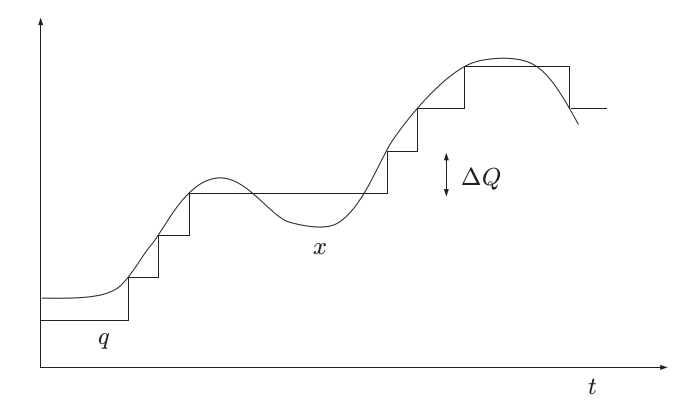
\includegraphics[scale=0.5]{histeresis1}
  \caption{Comportamiento de un modelo DEVS atómico}
   \label{fig:fig2-2}
\end{figure}

En la Figura \ref{fig:fig2-2} vemos la relación entrada-salida de una función de cuantificación de orden cero.

Las variables $q_j$ son llamadas variables cuantificadas y pueden ser vistas como una aproximación constante a trozos de la variable de estado correspondiente $x_j$. De la misma forma las componentes de $v(t)$ son aproximaciones constantes a trozos de las componentes correspondientes de $u(t)$. Los pasos de integración en los métodos de QSS sólo se producen cuando una variable cuantificada $q_j (t)$ cambia, esto es, cuando la variable de estado correspondiente $x_j (t)$ difiere de $q_j(t^{-})$ en un quantum. Ese cambio implica también que algunas derivadas de estado (aquellas que dependen de $x_j$ ) también son modificadas. 
	Luego, cada paso involucra un cambio en sólo una variable cuantificada y en algunas derivadas de estado. 
	Por lo tanto cuando un gran sistema ralo (o sparse) posee sólo actividad en unos pocos estados mientras que el resto del sistema se mantien	e intacto, los métodos de QSS explotan intrínsecamente este hecho realizando cálculos sólo donde y cuando ocurren los cambios.
	Otra ventaja importante de los métodos de QSS es que tratan las discontinuidades de una manera muy eficiente. Dependiendo del orden del método, las variables de estado siguen trayectorias lineal a trozos, parabólica a trozos o constante a trozos, la ocurrencia de una discontinuidad implica sólo algunos cálculos locales para re-computar las derivadas de estados que están directamente afectadas por ese evento.
Estas ventajas resultan en una aceleración notable en el tiempo de simulación contra los algoritmos de integración numérica clásicos. En modelos con discontinuidades frecuentes como sistemas de electrónica de potencia, los métodos de alto orden que veremos a continuación, pueden simular hasta 20 veces más rápido que los métodos convencionales.



\section{Modelica}

	Modelica es un lenguaje orientado a objetos desarrollado para describir de manera sencilla modelos de sistemas dinámicos eventualmente muy complejos.
	Además de las características básicas de todo lenguaje orientado a objetos, Modelica contiene herramientas específicas que permiten describir las relaciones
	constitutivas de los distintos componentes de cada modelo y las relaciones estructurales que definen la interacción entre dichos componentes.
	De esta manera, el lenguaje permite asociar cada componente de un sistema a una instancia de una clase de Modelica.
	Adicionalmente, los componentes típicos de los sistemas de distintos dominios de la física y de la técnica pueden agruparse en librerías de clases para ser
	reutilizados. De hecho, existe una librería estándar de clases de Modelica, que contiene los principales componentes básicos de sistemas eléctricos,
	mecánicos (traslacionales, rotacionales y multicuerpos), térmicos, state graphs, y diagramas de bloques. 
	Otras librerías (disponibles en la web) contienen componentes de sistemas hidráulicos, bond graphs, redes de petri, etc.
	Por otro lado, las herramientas que provee Modelica para expresar relaciones estructurales de un modelo permiten construir la estructura del mismo de una
	manera totalmente gráafica, lo que a su vez permite describir un sistema mediante un diagrama muy similar al del Sistema Físico Idealizado.
	Como con todo lenguaje, para poder simular un modelo descripto en Modelica es necesario utilizar un compilador. Actualmente existen tres compiladores
	más o menos completos de Modelica: Dymola, MathModelica y OpenModelica. Los dos primeros son herramientas comerciales que cuentan con interfaces
	gráficas para construir los modelos. OpenModelica es una herramienta libre, de código abierto.

\begin{listing}[H]    
	\caption{LotkaVolterra.mo}
	\inputminted{modelica}{src/LotkaVolterra.mo}
	\label{lst:LotkaVolterra.mo}
\end{listing} 


\section{$\mu$-Modelica}
El lenguaje $\mu$-Modelica tiene las siguientes restricciones con respecto a Modelica:

\begin{itemize}
 \item El modelo es plano, es decir no permite clases.
 \item Todas las variables pertenecen al tipo predefinido Real y solo hay tres categorías de variables: estado continuo, estado discreto y variables algebraicas.
 \item Los parámetros también son de tipo Real. 
 \item Arreglos están permitidos. Indices en los arreglos dentro de clausulas for están restringidos a la forma $\alpha \cdot i + \beta$, donde $\alpha$ y $\beta$ son expresiones enteras y $i$ es el indicie de la iteración.
 \item La sección de ecuaciones esta compuesta de :
 \begin{itemize}
	\item Definición de variables de estados : $der(x) =  f (x(t), d, a(t), t);$ ODE en forma explicita
	\item Definición algebraica : $(a_1 , \dots , a_n ) = g(x(t), d, a(t), t);$
 \end{itemize}
 con la restricción de que cada variable algebraica solo puede depender del estado y de variables algebraicas previamente definidas.
 
 \item Discontinuidades son expresadas solo con las clausulas $when$ y $elsewhen$ dentro de la sección $algorithm$. Las condiciones dentro de las dos clausulas solo pueden ser relaciones ($<$, $\leqslant$, $>$ $\geqslant$) y, dentro de la clausula, solo asignaciones de variables discretas y $reinit$ de estados continuos son permitidos
\end{itemize}

\section{Stand–Alone QSS solver}
Como mencionamos antes los métodos QSS de integración remplazan la discretización del tiempo de los métodos clásicos por una quantificación de las variables del sistema. De esta forma, estos métodos generan aproximaciones del sistema continuo y tienen algunas ventajas sobre sus contra partes clásicas.

La forma más simple de implementar algoritmos QSS es mediante el uso de un simulador DEVS, de hecho PowerDEVS implementa la totalidad de la familia de algoritmos QSS. Estas implementaciones aunque simples, son ineficientes, pues desperdician mucho poder computacional en sincronizar y transmisión de eventos.

Estas desventajas motivo el desarrollo del \emph{Stand–Alone QSS solver}, implementados como un conjunto de módulos en lenguaje C. Este implementa toda la familia de métodos QSS y permite que los modelos contengan discontinuidades de tiempo y estado.

Una dificultad impuesta por los métodos QSS es que hace uso de información estructural del modelo. Cada paso en un método QSS involucra un cambio en una variable de estado y en la derivada del estado que depende de el. Por lo que el modelo debe proveer no solo la expresión para calcular las derivadas del estado (como en un clásico ODE solver) pero además un matriz de incidencias para informar al solver que derivadas de estado han cambiado luego de cada paso.

Como sería muy incomodo para el usuario proveer esta información estructural, el solver tiene una interfaz que automáticamente obtiene la matriz de incidencia desde una definición estándar de modelos.

La interfaz permite al usuario describir el modelo utilizando un subconjunto del lenguaje estándar de Modelica ($\mu$Modelica) y automáticamente genera el código C del modelo incluyendo la estructura.



\section{Formalismo DEVS}
DEVS es un formalismo para modelar y analizar sistemas de eventos discretos (es decir, sistemas en los cuales en un lapso finito de tiempo, ocurren una cantidad finita de eventos).
Un modelo DEVS puede ser visto como un autómata que procesa una serie de eventos de entrada y genera una serie de eventos de salida. Este procesamiento está regido por la estructura interna de cada una de las partes que componen el modelo general.
Un modelo DEVS está descripto por dos clases de componentes, modelos atómicos y modelos acoplados.

\subsection{Atómicos}
Un modelo atómico representa la unidad \quotes{indivisible} de especificación, en el sentido que es la pieza fundamental y más básica de un modelo DEVS. Formalmente un modelo atómico está conformado por la 7-upla:

\begin{equation} 
(X, Y, S, \delta_{int} , \delta_{ext}, \lambda, t_{a}) \mbox{ donde :}
\end{equation}

\begin{itemize}
\item $X$ es el conjunto de valores de entrada que acepta el modelo atómico, es decir un evento de entrada tiene como valor un elemento del conjunto X.
\item $Y$ es el conjunto de valores de los eventos de salida que puede emitir el modelo atómico.
\item $S$ es el conjunto de estados internos del modelo, en todo momento el atómico está en un estado dado, que es un elemento del conjunto S.
\item $ta$ es una función $S \to R^{+}_{0}$ , que indica cuánto tiempo el modelo atómico permanecerá en un estado dado, si es que no se recibe ningún evento de entrada. Esta función es \emph{Función de Avance de Tiempo}.
\item $\delta_{int}$ es una función $S \to S$, que indica la dinámica del sistema en el momento que el modelo atómico realiza una transición interna. Sería el análogo a una tabla de transición en otros autómatas, es la \emph{Función de Transición Interna}.
\item $\delta_{ext}$ es una función $(S \times \mathcal{P}(R^{+}_{0}) \times X) \to S$, que indica el cambio de estado ante la presencia de un evento externo, esta es la \emph{Función de Transición Externa}.
\item $\lambda$ es una función $S \to Y$ que indica qué evento se debe emitir al salir de un estado dado, es \emph{Función de Salida}.
\end{itemize}

Los conjuntos $S$, $X$ e $Y$ son arbitrarios, y en general infinitos. Cada posible estado $s$ ($s \in S$) tiene asociado un Avance de Tiempo calculado por la Función de Avance de Tiempo $ta(s)$.
En la Figura \ref{fig:fig2-5} vemos la evolución de un modelo atómico. Si el estado toma el valor $s_1$ en el tiempo $t_1$ , tras $ta(s_1)$ unidades de tiempo (o sea, en tiempo $ta(s_1 ) + t_1 )$ el sistema realizará una transición interna yendo a un nuevo estado $s_2$ dado por $s_2 = \delta_{int} (s_1 )$. La función $\delta_{int}$ se llama Función de Transición Interna.

Cuando el estado va de $s_1$ a $s_2$ se produce también un evento de salida con valor $y_1 = \lambda(s_1)$. La función $\lambda (\lambda : S \to Y )$ se llama Función de Salida. Así, las funciones $ta$, $\delta_{int}$ y $\lambda$ definen el comportamiento autónomo de un modelo DEVS.

Cuando llega un evento de entrada, el estado cambia instantáneamente. El nuevo valor del estado no sólo depende del valor del evento de entrada sino también del valor anterior del estado y del tiempo transcurrido desde la última transición.

Si el sistema llega al estado $s_3$ en el instante $t_3$ y luego llega un evento de entrada en el instante $t_3 + e$ con un valor $x_1$ , el nuevo estado se calcula como $s_4 = \delta_{ext} (s_3 , e, x_1 )$ (notar que $ta(s_3 ) > e$). En este caso se dice que el sistema realiza una transición externa. La función $\delta_{ext}$ se llama Función de Transición Externa. Durante una transición externa no se produce ningún evento de salida.
\begin{figure}[!htbp]
  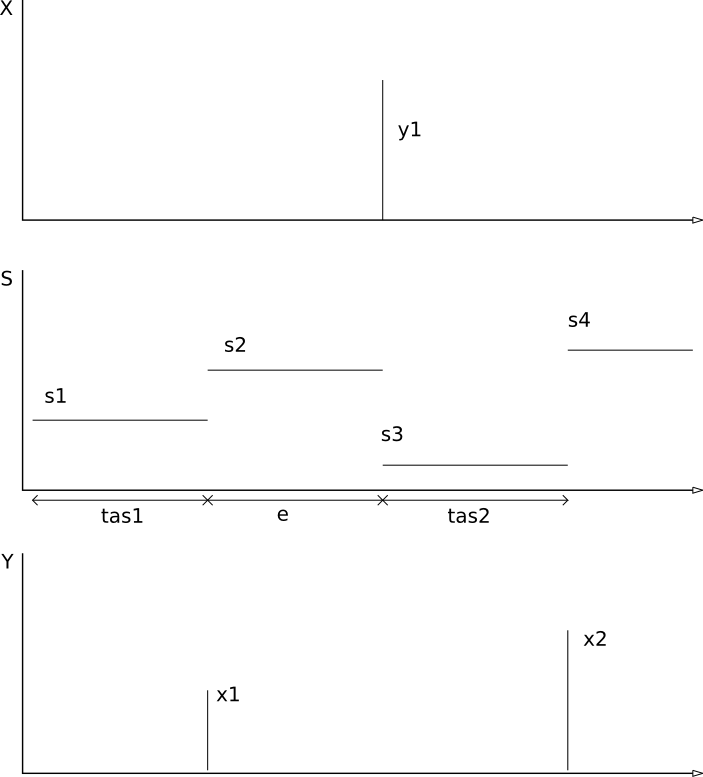
\includegraphics[scale=0.5]{devs-atomic}
  \caption{Comportamiento de un modelo DEVS atómico}
   \label{fig:fig2-5}
\end{figure}

\subsection{Acoplados}
La descripción de un sistema puede ser completamente realizada utilizando modelos atómicos, aunque esto resulta un poco incómodo y confuso. Los conjuntos de estados y las funciones de transición se vuelven inmanejables en sistemas complejos, y nunca podemos asegurar haber cubierto todos los posibles estados.
Para abordar este problema, el formalismo DEVS introduce lo que se llaman modelos acoplados, que es una forma de agrupar modelos DEVS y generar nuevos modelos a partir de este agrupamiento.
Hay dos formas de acoplamiento, la más general, en la cual se utilizan funciones de traducción entre los sub–sistemas y otra clase que adopta el uso de puertos para la comunicación entre sub–sistemas. Aunque estas dos formas son equivalentes entre sí, describiremos la segunda clase, ya que es la más simple y es la utilizada en el presente trabajo.
Formalmente un modelo acoplado está representado por la octo-upla:

\begin{equation}
N = (X_N , Y_N , D, {M_d }, EIC, EOC, IC, Select)
\end{equation}

donde cada componente es:
\begin{itemize}
\item $X_N$ es el conjunto de eventos de entrada al modelo acoplado, representado por el producto cartesiano del conjunto de puertos de entrada $InPorts$ y el conjunto de posibles valores para cada puerto. O sea un evento de entrada al modelo acoplado está representado por un par $(p, v)$ donde $p \in InPorts$ y $v \in X_p$ .

\item $Y_N$ es el conjunto de eventos que el modelo puede emitir. Es un elemento del producto cartesiano entre el conjunto de puertos de salida $OutPorts$ y el conjunto de posibles valores para este puerto, o sea un evento de salida del modelo acoplado está representado por un par $(p, v)$ donde $p \in OutPorts$ y $v \in Y_p$.

\item $D$ es el conjunto de los índices a los modelos DEVS (atómicos y acoplados) que conforman este modelo. 

\item ${M_d}$ es el conjunto de los modelos atómicos y/o acoplados (son justamente los modelos que \quotes{acopla} o \quotes{agrupa} este modelo acoplado).

\item EIC y EOC son el conjuntos de conexiones entre los modelos internos y los puertos del modelo acoplado:
      \begin {itemize}
          \item EIC (o External Input Coupling) son las conexiones de entrada al acoplado, es decir, conecta un puerto de entrada del acoplado con un puerto de entrada de un modelo perteneciente al acoplado.
          \item EOC (o External Output Coupling) son las conexiones de salida del acoplado. Conecta un puerto de salida de un modelo interno del acoplado con un puerto de salida del acoplado.  
     \end{itemize}

\item $IC$ representa las conexiones internas del modelo acoplado.

\item Select es una función $(\mathcal{P}((D)) \to D)$ que decide qué modelo realizará primero su transición interna, si se da el caso de eventos simultáneos. Es una función de \quotes{desempate} que en ciertos modelos es necesaria.
\end{itemize}

Formalmente:
\begin{align*}
EIC \in& \{((N, ip_N ), (d, ip_d )) | ip_N \in InPorts, d \in D, ip d \in InPorts_d \} \\
EOC \in& \{((d, op_d ), (N, op_N ))  | op_N \in OutPorts, d \in D, op d \in OutPorts_d \}
\end{align*}
donde N es el modelo acoplado.
\begin{equation*}
IC \in \{((a, ip_a ), (b, ip_b )) | a, b \in D, ip a \in OutPorts_a , ip_b \in InPorts_b \}
\end{equation*}
donde no se permite que $a = b$.

$InPorts$ y $Outports$ son conjuntos que describen los posibles puertos de entrada y salida respectivamente. En general se utilizan números enteros para representar los puertos posibles por lo cual $InPorts = \mathbb{N}$ y $Outports = \mathbb{N}$. Los modelos acoplados son en sí mismos modelos DEVS válidos; formalmente el acoplamiento (como lo definimos antes) es una operación cerrada sobre el conjunto de modelos DEVS. Acoplar modelos DEVS forma nuevos modelos DEVS. Sin esta cualidad el acoplamiento resultaría inútil desde del punto de vista del formalismo. También trae muchas ventajas a la hora de describir modelos DEVS y a la hora de simularlos. El acoplamiento da lugar a una estructura jerárquica de desarrollo.

$EIC$, $EOC$ y $IC$ son conjunto de pares, de pares, como se encuentran conectados los modelos (atómicos o acoplados) a través de sus puertos con los puertos de entrada, salida y con otros modelos (atómicos o acoplados) respectivamente. Tanto los puertos como los modelos son señalados por números dentro de PowerDEVS, por lo que estos conjuntos estan comprendidos por elementos de la forma $(m_a, p_a), (m_b, p_b)$, donde $m_a$ y $m_b$ son modelos (atomicos o no) en el actual modelo y $p_a$ y $p_b$ son sus correspondientes puertos.

\begin{figure}[H]

\begin{minipage}{0.5\textwidth}
\centering
\TBox{%
  \TBox[]{Acoplado2 \\ \TBox{Acoplado1 \\ \TBox[]{Atómico1}\TBox{Atómico2} } \TBox{Atómico3} }}
\end{minipage}\hfill
\begin{minipage}{0.5\textwidth}
\centering

\tikzstyle{every node}=[draw=black,thick,anchor=west]
\tikzstyle{selected}=[draw=red,fill=red!30]
\tikzstyle{optional}=[dashed,fill=gray!50]
\begin{tikzpicture}[%
  grow via three points={one child at (0.5,-0.7) and
  two children at (0.5,-0.7) and (0.5,-1.4)},
  edge from parent path={(\tikzparentnode.south) |- (\tikzchildnode.west)}]
  \node {Root-Coordinator}
    child { node {Acoplado2}		
    child { node {Acoplado1}
      child { node {Atómico1}}
      child { node {Atómico2}}
    }
    child [missing] {}				
    child [missing] {}				
    child [missing] {}				
    child { node {Atómico3}}};
\end{tikzpicture}
\end{minipage}

\caption{Ejemplo de un modelo jerarquico.}

\end{figure}


\subsection{Modelos DEVS parametrizados}
Definirmos primero los modelos DEVS parametrizados como un paso previo hacia el formalismo DEVS vectorial (Vectorial DEVS or VECDEVS), el cua es una herramienta que nos facilitará representar modelos de gran escala en forma gráfica, en particular este formalismo se encuentra implementado en la herramienta PowerDEVS.

Dado un modelo DEVS atómico $M$ obtenemos un Modelo DEVS Parametrizado:
\begin{equation}
M (p) = \{X, Y, S, \delta_{int}, \delta_{ext} ,\lambda , ta, p\}
\end{equation}

donde $p \in P$ es un parámetro que pertenece a un conjunto de parámetros arbitrario tal que $\delta_{int}$ , $\delta_{ext}$ , $\lambda$ y $ta$ dependen también de $p$.
Notar que dos modelos DEVS $M (p_1 )$, $M (p_2 )$ con $p_1 \neq p_2$ pueden exhibir distintos comportamientos aunque compartan los mismos conjuntos de entrada, salida y de estados ($X$, $Y$ , y $S$, respectivamente).

\subsection{Modelos Vectoriales}
Dado el modelo escalar DEVS Parametrizado:
\begin{equation}
M (p) = \{X, Y, S, \lambda_{int} , \lambda_{ext} , \lambda, ta, p\}
\end{equation}

definimos un modelo Vectorial DEVS como la estructura:
\begin{equation}
V_D = \{N, X_V, Y_V, P, \{M_i\}\},
\end{equation}
donde:
\begin{itemize}
\item $N \in \mathbb{N}$ es la dimensión del modelo vectorial.

\item $X_V = X \times Index \bigcup \{-1\}$ es el conjunto de eventos de entradas vectorial donde $X$ es el conjunto de eventos de entrada del modelo escalar e $Index = {1, \ldots , N }$ es el conjunto de índices que indican cuál de los modelos DEVS atómicos recibirá el evento.

\item $Y_V = Y \times Index$ es el conjunto de eventos de salida vectorial donde $Y$ es el conjunto de eventos de salida del modelo escalar e $Index = {1, \ldots , N }$ es el conjunto de índices que indica que modelo escalar de los $N$ , emitió el evento. 

\item $P$ es un conjunto de parámetros arbitrario.

\item Para cada índice $i \in Index$, $p(i) \in P$ es un parámetro y $M_i = M (p(i))$ es el modelo DEVS Parametrizado escalar.
\end{itemize}

\subsubsection{Interfaz entre DEVS Vectorial y DEVS}
Para conectar bloques vectoriales y bloques escalares es necesarios bloques que hagan de interfaz entre los dos formalismo, además, introducimos un bloque necesario para realizar modelos más complejos y conectar los diferentes componentes de un modelo vectorial entre sí.

\begin{itemize}
	\item Escalar a Vector (Scalar to Vector): Este boque simplemente agrega al indice $i$ al evento escalar que recive, transformándolo en un evento vectorial. Este modelo también posee un comportamiento especial para enviar el mismo evento en todas las componentes vectorial al mismo tiempo, cuando $i = -1$, cada evento de entrada es trasmitido para todas las componentes del vector salida.
	\item Vector a escalar (Vector to Scalar): Este bloque tiene un parámetro $i$ que contiene el índice del vector de eventos a retransmitir, cuando recibe un evento con indice $j=i$, remueve el indice y retransmite el evento escalar.
	\item Index Shift: El modelo más simple es el Index Shift. Cuando se recibe un evento con el valor $(x,i)$, envia un evento de salida $(x, i+sh)$, donde $sh$ es un parámetro entero.
\end{itemize}

En este trabajo todos estos bloques se la ha agregado la dimensión $N$ como parámetro, esto es necesario para realizar la conversión de los modelos, de forma que no existan desconexiones a nivel Modelica, lo cual se reflejaría en un modelo con menos ecuaciones que variables, es decir un modelo no balanceado.
	 
\section{PowerDEVS}
PowerDEVS es un programa, concebido para ser utilizado por expertos programadores DEVS, así como usuarios finales que solo quieren conectar bloques y simular.

PowerDEVS esta compuesto por varios programas independientes:
\begin{itemize}
\item El \emph{editor de modelos}, es desde el punto de vista del usuario, el principal programa de PowerDEVS, pues provee la interfaz gráfica y enlaces para las demás aplicaciones. 
Además de construir, manejar modelos y librerías, permite lanzar las simulaciones (lanzando el \emph{Pre procesador}) y editar los bloques elementales hasta su definición atómica de modelo (invocando el \emph{Editor Atómico}).
La ventana principal de \emph{Editor de Modelo} permite al usuario crear y abrir modelos y librerías. También permite a las librerías ser exploradas y los bloques arrastrados de las librerías a los modelos.
También existen algunas características avanzadas que pueden ser manejadas desde la ventana principal como establecer cual es la librería activa, y configurar las barras de herramientas y menúes para invocar aplicaciones externas.
La ventana del Modelo provee todas las funcionalidades típicas para la edición gráfica para poder copiar, cambiar el tamaño, rotar, etc. mientras que las conexiones pueden ser dibujadas entre los diferentes puertos.
La ventana de Edición de Bloques, nos permite configurar la apariencia gráfica y elegir los parámetros del bloque y, en el caso de los modelos atómicos, seleccionar el archivo que contiene el código asociado con la definición DEVS.

\item El \emph{Editor de Modelos Atómico} facilita la edición del código C++ correspondiente a cada modelo atómico DEVS, el usuario solo debe definir las variables que forman el estado y la salida del modelo DEVS. Luego, el código C++ de la transición de avance de tiempo y la función de salida deben se completados. Hay dos ventanas adicionales init y exit, donde se puede completar con código que sera ejecutado al inicio y fin de la simulación.
Cuando el modelo se guarda, el código es guardado en los archivos .cpp y .h. 

\item El \emph{Pre procesador}, toma un archivo .pdm (o .pds) producido por el \emph{Editor de Modelos} y produce el programa que corre la simulación. Básicamente traduce el archivo .pdm a un archivo de cabecera .h que enlaza el simulador y el coordinador de acuerdo a la estructura del modelo pasando además los parámetros definidos para el modelo.
El \emph{Pre procesador}, además produce un makefile (Makefile.include) el cual invoca el compilador para generar el programa que implementa la simulación.

\item La \emph{interfaz de simulación}, que corre el programa que implementa la simulación y permite variar parámetros de la simulación como tiempo final, números de simulación a ejecutar, y el modo de simulación (normal, cronometrada, pasa o paso, etc.).

\item Una instancia de Scilab, que actua como un espacio de trabajo, donde los parámetros pueden ser leídos, y los resultados pueden ser exportados.
\end{itemize}

